% Compiler: LaTeX => PDF

\documentclass{beamer}

\usepackage[ngerman]{babel}
\usepackage[utf8]{inputenc}

%\usepackage{multimedia}
\usepackage{graphicx}
\usepackage[nolist]{acronym}

\usepackage{stackengine}
\usepackage{array}

\usepackage{enumitem}

\setitemize{label=\usebeamerfont*{itemize item}%
  \usebeamercolor[fg]{itemize item}
  \usebeamertemplate{itemize item}}

\title{Shape from X}
\subtitle{X $\in \{$ Motion, Shading, Texture $\}$}
%\subtitle{Schwerpunkte: Shape from Motion, \\ Shape from Shading, Shape from Texture}
\author{Dennis Wagner, \\ Johannes Spangenberg, \\ Leroy Kramer}
%\date{\today}
\date{04.12.2014}

% add page number
\setbeamertemplate{footline}[frame number]

\begin{document}


\begin{acronym}[SIFT]
	\acro{SIFT}{Scale-invariant feature transform}
	\acro{KLT}{Kanade–Lucas–Tomasi}
\end{acronym}


\frame{\titlepage} 


\begin{frame}
	\frametitle{Gliederung}
	\tableofcontents
\end{frame} 


\section{Einleitung} 
\begin{frame}
	\frametitle{Shape from X}
	\framesubtitle{Einleitung}
	
	\begin{itemize}
		\item 3D Objekt aus einem oder mehreren Bildern rekonstruieren
		\item verschiedene Verfahren
		\begin{itemize}
			\item \textbf{Motion}
			\item \textbf{Shading}
			\item \textbf{Texture}
			\item Zoom
			\item Focus
			\item Stereo
			\item ...
		\end{itemize}
		\item Günstige Quelle von dreidimensionalen Strukturen.
		\begin{itemize}
			\item Computervisualisierung (Spiele, \dots)
		\end{itemize}
		
	\end{itemize}
\end{frame}

% ---------------------------------------------------------------------------- %

\section{Shape from Motion}

\begin{frame}	
	\center	\huge Shape from Motion
\end{frame}

\begin{frame}
	\frametitle{Shape from Motion}
	\framesubtitle{Einleitung}

	\begin{description}
		\item[Eingabe:] Reihe von Bildern einer Szene aus verschiedenen Perspektiven
		\item[Ausgabe:] Dreidimensionale Rekonstruktion der Szene
	\end{description}

	\begin{block}{Motivation}
		\begin{itemize}
			\item Konstruktion von Modellen zur Präsentation
			\item Einfache Vermessung größerer Gebiete
		\end{itemize}
	\end{block}
\end{frame}


\subsection{Verarbeitungsschritte}
\begin{frame}
	\frametitle{Shape from Motion}
	\framesubtitle{Verarbeitungsschritte}

	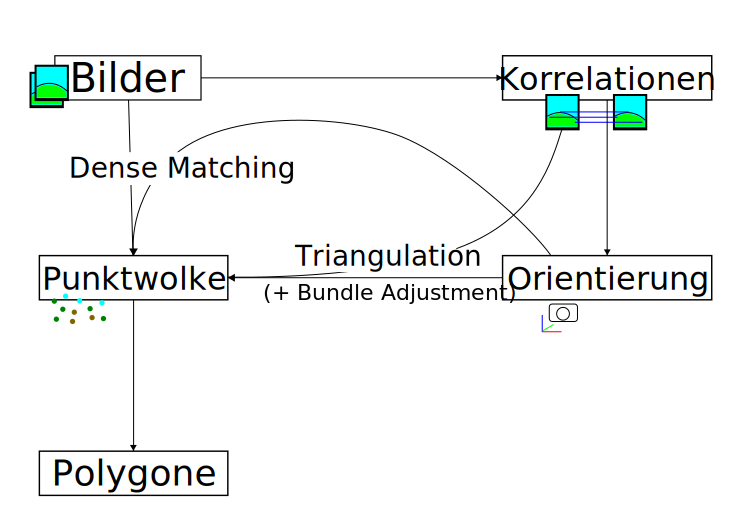
\includegraphics[width=\linewidth]{includes/shape-from-motion_process}
\end{frame}


\begin{frame}
	\frametitle{Shape from Motion}
	\framesubtitle{Korrelationen finden}

	\begin{figure}
		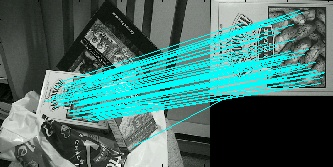
\includegraphics[width=\linewidth]{includes/sift}\\
		{\scriptsize Fig. 1.1: Beispielergebnis für SIFT}
	\end{figure}
\end{frame}


\begin{frame}
	\frametitle{Shape from Motion}
	\framesubtitle{Verarbeitungsschritte}

	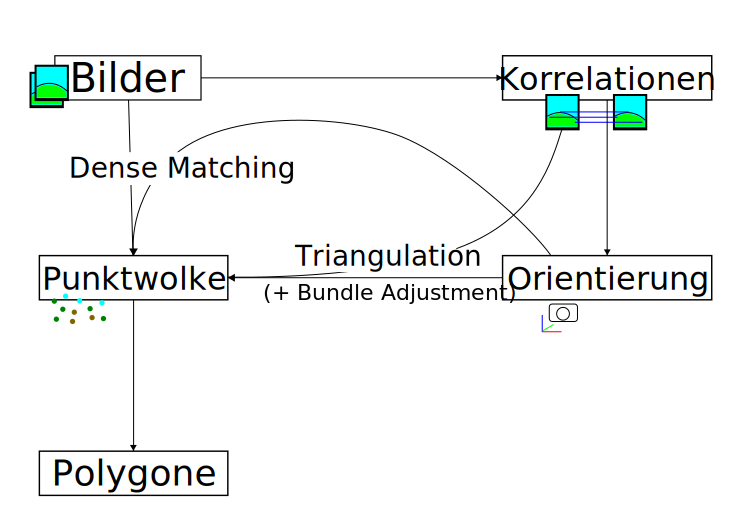
\includegraphics[width=\linewidth]{includes/shape-from-motion_process}
\end{frame}


\begin{frame}
	\frametitle{Shape from Motion}
	\framesubtitle{Orientierung berechnen}

	\vspace{1em}
	Die Orientierungsberechnung benutzt das Model der Lochkamera (engl. \textit{pinhole camera}) und die Epipolargeometrie.

	\begin{figure}
		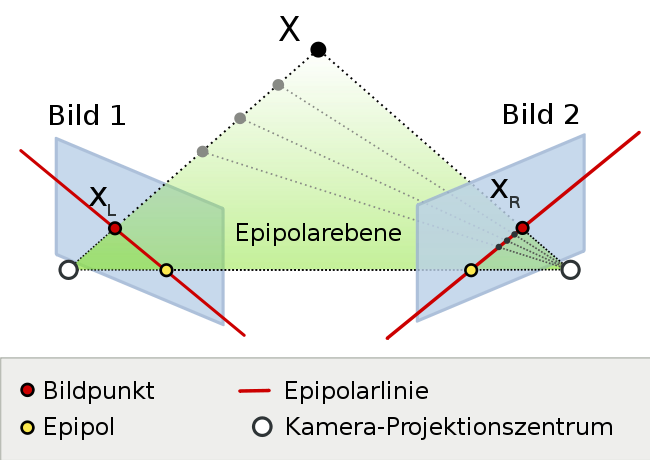
\includegraphics[width=217pt]{includes/Epipolargeometrie3}\\
		{\scriptsize Fig. 1.2: Epipolargeometrie}
	\end{figure}
\end{frame}


\begin{frame}
	\frametitle{Shape from Motion}
	\framesubtitle{Verarbeitungsschritte}

	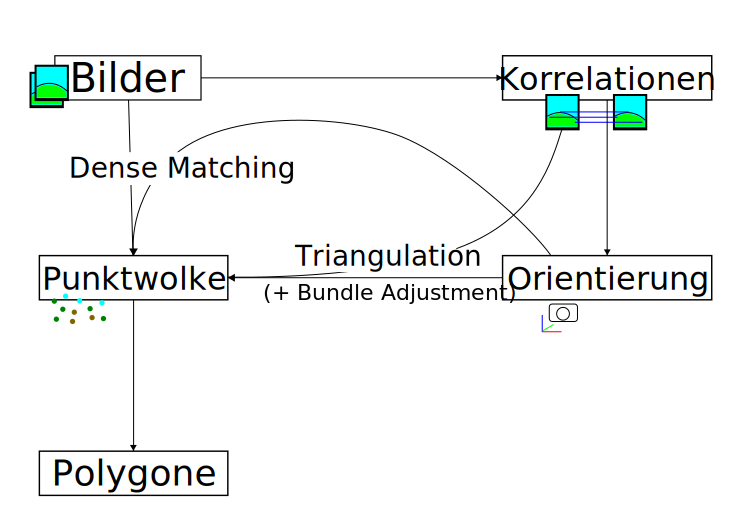
\includegraphics[width=\linewidth]{includes/shape-from-motion_process}
\end{frame}


\begin{frame}
	\frametitle{Shape from Motion}
	\framesubtitle{Dense Matching}

	\begin{figure}
		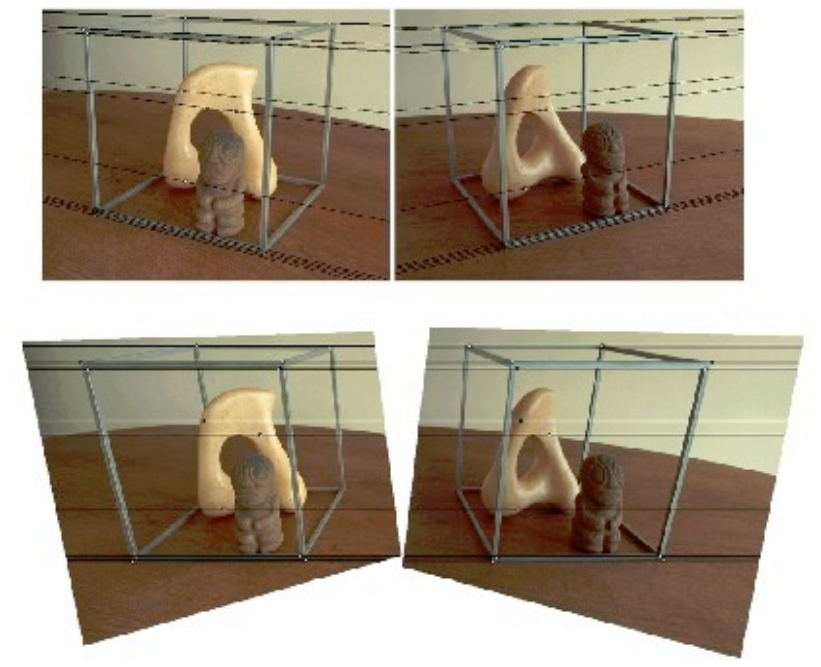
\includegraphics[width=0.8\linewidth]{includes/dense-matching}\\
		{\scriptsize Fig. 1.3: Ausrichtung angleichen}
	\end{figure}
\end{frame}

% ---------------------------------------------------------------------------- %

\section{Shape from Shading}

\begin{frame}	
	\center	\huge Shape from Shading
\end{frame}

\subsection{Ansätze}
\begin{frame}
	\frametitle{Shape from Shading}
	\framesubtitle{Ansätze}
	
	
	\begin{tabular}{lm{0.12\linewidth}m{0.12\linewidth}m{0.12\linewidth}m{0.12\linewidth}}
		\begin{tabular}{l} Original \end{tabular} &
		\begin{tabular}{c} 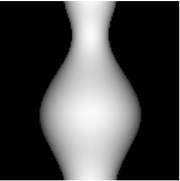
\includegraphics[width=1.2\linewidth]{includes/vergleich/vorlage/vorlage_vase_001}  \end{tabular} & 
		\begin{tabular}{c} 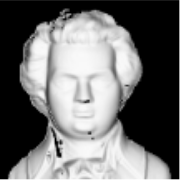
\includegraphics[width=1.2\linewidth]{includes/vergleich/vorlage/vorlage_mozart_001}  \end{tabular} &
		\begin{tabular}{c} 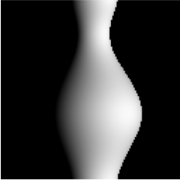
\includegraphics[width=1.2\linewidth]{includes/vergleich/vorlage/vorlage_vase_101}  \end{tabular} & 
		\begin{tabular}{c} 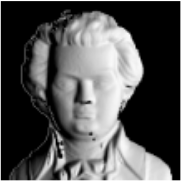
\includegraphics[width=1.2\linewidth]{includes/vergleich/vorlage/vorlage_mozart_101}  \end{tabular} \\
		\begin{tabular}{l} Minimierung \\ (Lee \& Kuo) \end{tabular}  &
		\begin{tabular}{c} 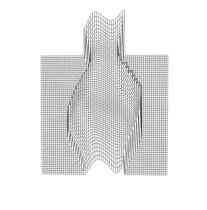
\includegraphics[width=1.2\linewidth]{includes/vergleich/lee_kuo/lee_kuo_vase_001}  \end{tabular} & 
		\begin{tabular}{c} 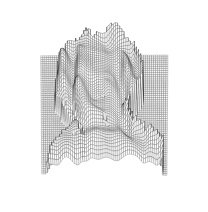
\includegraphics[width=1.2\linewidth]{includes/vergleich/lee_kuo/lee_kuo_mozart_001}  \end{tabular} &
		\begin{tabular}{c} 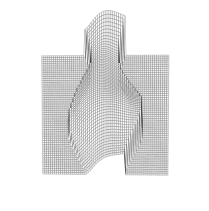
\includegraphics[width=1.2\linewidth]{includes/vergleich/lee_kuo/lee_kuo_vase_101}  \end{tabular} & 
		\begin{tabular}{c} 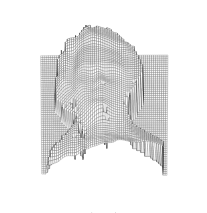
\includegraphics[width=1.2\linewidth]{includes/vergleich/lee_kuo/lee_kuo_mozart_101}  \end{tabular} \\
		\begin{tabular}{l} Ausbreitung \\ (Bichsel \& Pentland) \end{tabular} &
		\begin{tabular}{c} 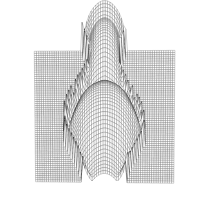
\includegraphics[width=1.2\linewidth]{includes/vergleich/bichsel_pentland/bichsel_pentland_vase_001}  \end{tabular} &
		\begin{tabular}{c} 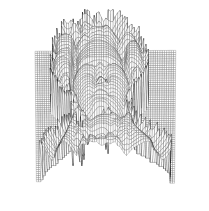
\includegraphics[width=1.2\linewidth]{includes/vergleich/bichsel_pentland/bichsel_pentland_mozart_001}  \end{tabular} &
		\begin{tabular}{c} 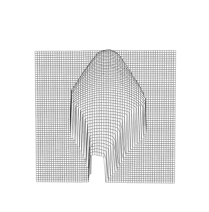
\includegraphics[width=1.2\linewidth]{includes/vergleich/bichsel_pentland/bichsel_pentland_vase_101}  \end{tabular} &
		\begin{tabular}{c} 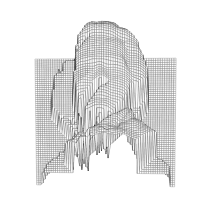
\includegraphics[width=1.2\linewidth]{includes/vergleich/bichsel_pentland/bichsel_pentland_mozart_101}  \end{tabular} \\
		\begin{tabular}{l} Lokal \\ (Lee \& Rosenfeld) \end{tabular} &
		\begin{tabular}{c} 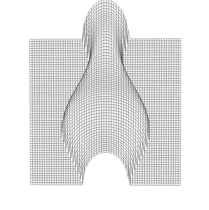
\includegraphics[width=1.2\linewidth]{includes/vergleich/lee_rosenfeld/lee_rosenfeld_vase_001}  \end{tabular} &
		\begin{tabular}{c} 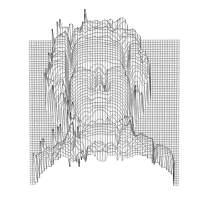
\includegraphics[width=1.2\linewidth]{includes/vergleich/lee_rosenfeld/lee_rosenfeld_mozart_001}  \end{tabular} &
		\begin{tabular}{c} 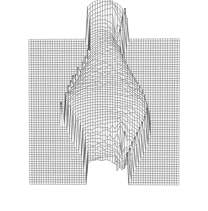
\includegraphics[width=1.2\linewidth]{includes/vergleich/lee_rosenfeld/lee_rosenfeld_vase_101}  \end{tabular} &
		\begin{tabular}{c} 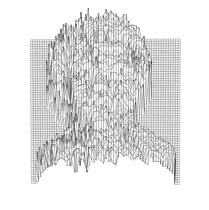
\includegraphics[width=1.2\linewidth]{includes/vergleich/lee_rosenfeld/lee_rosenfeld_mozart_101}  \end{tabular} 
\end{tabular}
\begin{center} \scriptsize Fig. 2.1 \end{center}
	
\end{frame}

\begin{frame}
	\frametitle{Shape from Shading}
	\framesubtitle{Ansätze}
	
	\begin{tabular}{lm{0.16\linewidth}m{0.16\linewidth}m{0.16\linewidth}}
		\begin{tabular}{l} Original \end{tabular} &
		\begin{tabular}{c} 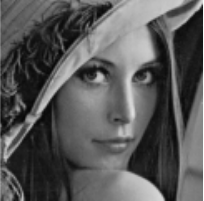
\includegraphics[width=\linewidth]{includes/vergleich/vorlage/vorlage_lenna}  \end{tabular} & 
		\begin{tabular}{c} 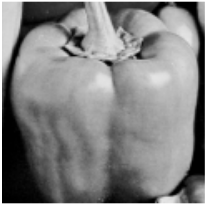
\includegraphics[width=\linewidth]{includes/vergleich/vorlage/vorlage_pepper}  \end{tabular} &
		\begin{tabular}{c} 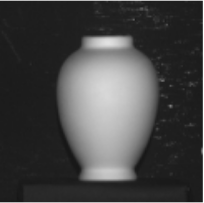
\includegraphics[width=\linewidth]{includes/vergleich/vorlage/vorlage_vase}  \end{tabular} \\
		\begin{tabular}{l} Minimierung \\ (Lee \& Kuo) \end{tabular}  &
		\begin{tabular}{c} 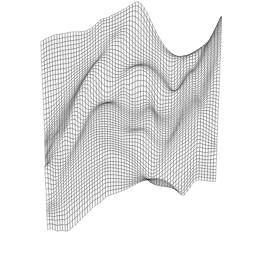
\includegraphics[width=\linewidth]{includes/vergleich/lee_kuo/lee_kuo_lenna}  \end{tabular} & 
		\begin{tabular}{c} 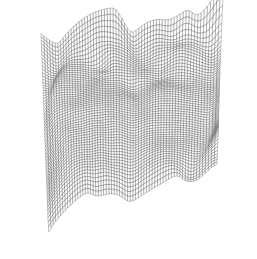
\includegraphics[width=\linewidth]{includes/vergleich/lee_kuo/lee_kuo_pepper}  \end{tabular} &
		\begin{tabular}{c} 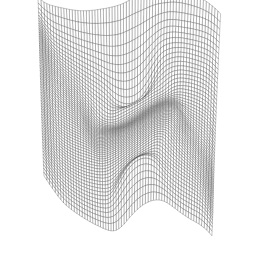
\includegraphics[width=\linewidth]{includes/vergleich/lee_kuo/lee_kuo_vase}  \end{tabular} \\
		\begin{tabular}{l} Ausbreitung \\ (Bichsel \& Pentland) \end{tabular} &
		\begin{tabular}{c} 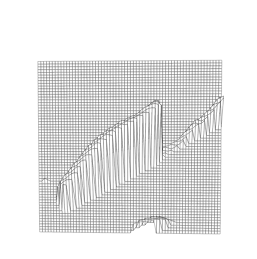
\includegraphics[width=\linewidth]{includes/vergleich/bichsel_pentland/bichsel_pentland_lenna}  \end{tabular} & 
		\begin{tabular}{c} 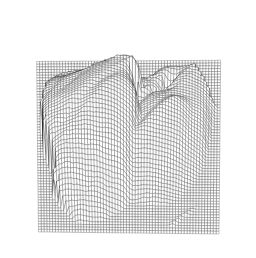
\includegraphics[width=\linewidth]{includes/vergleich/bichsel_pentland/bichsel_pentland_pepper}  \end{tabular} &
		\begin{tabular}{c} 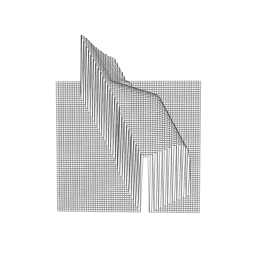
\includegraphics[width=\linewidth]{includes/vergleich/bichsel_pentland/bichsel_pentland_vase}  \end{tabular} \\
		\begin{tabular}{l} Lokal \\ (Lee \& Rosenfeld) \end{tabular} &
		\begin{tabular}{c} 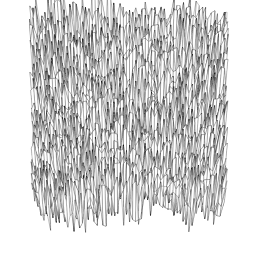
\includegraphics[width=\linewidth]{includes/vergleich/lee_rosenfeld/lee_rosenfeld_lenna}  \end{tabular} &
		\begin{tabular}{c} 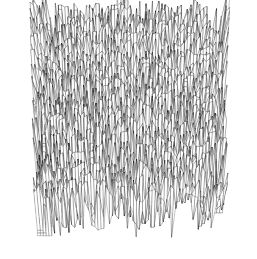
\includegraphics[width=\linewidth]{includes/vergleich/lee_rosenfeld/lee_rosenfeld_pepper}  \end{tabular} &
		\begin{tabular}{c} 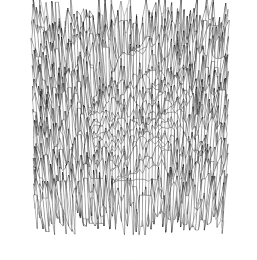
\includegraphics[width=\linewidth]{includes/vergleich/lee_rosenfeld/lee_rosenfeld_vase}  \end{tabular} 
	\end{tabular}
	
\begin{center} \scriptsize Fig. 2.2 \end{center}
\end{frame}

\subsection{Probleme}
\begin{frame}
	\frametitle{Shape from Shading}
	\framesubtitle{Probleme}
	
	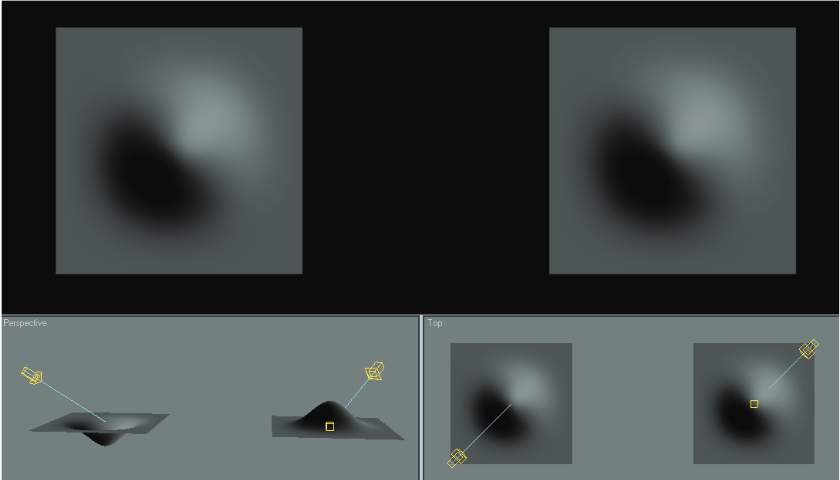
\includegraphics[width=\linewidth]{includes/shading_problem}\\
	\begin{center} \scriptsize Fig. 2.3 \end{center}
\end{frame}

% ---------------------------------------------------------------------------- %

\section{Shape from Texture}

\begin{frame}
	\center \huge Shape from Texture
\end{frame}

\frame{
	\frametitle{Shape from Texture}
	\framesubtitle{Einleitung}
	\begin{figure}
	\stackunder{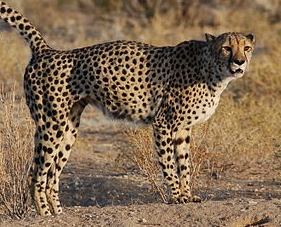
\includegraphics[width=99px, height = 80px]{includes/sft_texture_2}}{\scriptsize Fig. 3.1}
	\stackunder{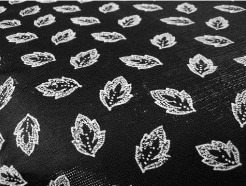
\includegraphics[width=105px, height = 80px]{includes/sft_texture_1}}{\scriptsize Fig. 3.2}
	\end{figure}

	\begin{itemize}
		\item Objekt mit texturierter Oberfläche rekonstruieren
		\item Textur besteht aus sich wiederholenden Texturelementen (Texel)
		\item Unterscheidung zwischen globalen und lokalen Verfahren
	\end{itemize}
}

\frame{
	\frametitle{Shape from Texture}
	\framesubtitle{Normale berechnen}
	\begin{figure}
	\stackunder{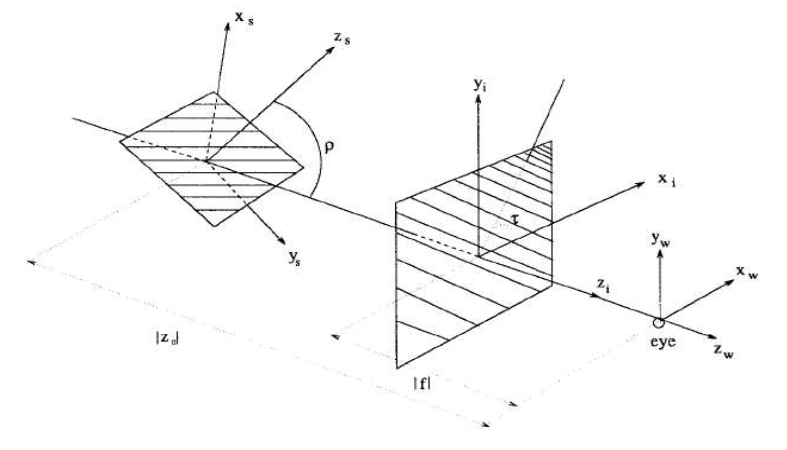
\includegraphics[width=230px, height = 120px]{includes/sft_slant-tilt}}{\scriptsize Fig. 3.3}
	\end{figure}
	\begin{itemize}
		\item slant $\rho$: Winkel zwischen $z_s$ und $z_i$\\
		\item tilt $\tau$: Winkel zwischen Projektion von $z_s$ auf Bildebene und $x_i$\\
		\item Normale: $z_s = \begin{pmatrix}
			\sin \rho \cos \tau\\
			\sin \rho \sin \tau\\
			\cos \rho
			\end{pmatrix}$
	\end{itemize}
}

\frame{
	\frametitle{Shape from Texture}
	\framesubtitle{Ergebnis}
	
	\begin{figure}
	\stackunder{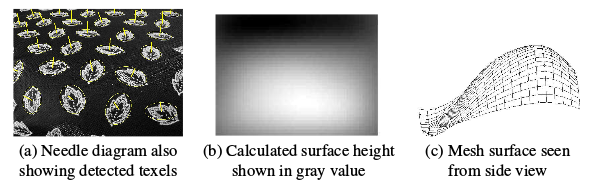
\includegraphics[width=300px, height = 96px]{includes/sft_result}}{\scriptsize Fig. 3.4}
	\stackunder{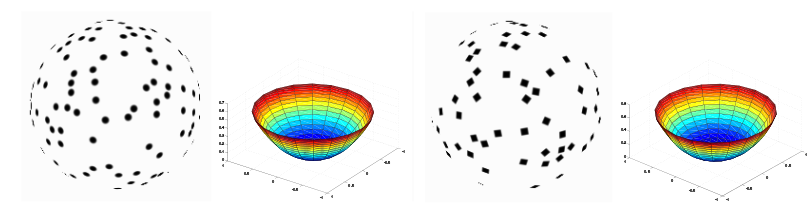
\includegraphics[width=300px, height = 81px]{includes/sft_result2}}{\scriptsize Fig. 3.5}
	\end{figure}
}



\begin{frame}	
	\frametitle{Shape from X}
	\center \LARGE Vielen Dank für eure Aufmerksamkeit!
\end{frame}
% ---------------------------------------------------------------------------- %

\section{Quellenverzeichnis}
\begin{frame}
	\frametitle{Quellenverzeichnis}
	\framesubtitle{Shape from Motion}
	
	\begin{tiny}
	\begin{enumerate}[label={[1.\arabic*]}]
		%\item \href{http://tu-dresden.de/die\_tu\_dresden/fakultaeten/fakultaet\_forst\_geo\_und\_hydrowissenschaften/fachrichtung\_geowissenschaften/ipf/photogrammetrie/elearning/software\_sfm}{http://tu-dresden.de/die\_tu\_dresden/fakultaeten/fakultaet\_forst\_geo\_und\_hydrowissenschaften/fachrichtung\_geowissenschaften/ipf/photogrammetrie/elearning/software\_sfm}
		\item
		\href{http://de.wikipedia.org/wiki/Bildregistrierung}{http://de.wikipedia.org/wiki/Bildregistrierung}
		\item
		\href{http://de.wikipedia.org/wiki/Epipolargeometrie}{http://de.wikipedia.org/wiki/Epipolargeometrie}
		\item
		\href{http://en.wikipedia.org/wiki/Scale-invariant_feature_transform}{http://en.wikipedia.org/wiki/Scale-invariant\_feature\_transform}
		\item
		% Irgend sowas ueber SfM
		\href{http://mi.eng.cam.ac.uk/~cipolla/publications/contributionToEditedBook/2008-SFM-chapters.pdf}{http://mi.eng.cam.ac.uk/$\sim$cipolla/publications/contributionToEditedBook/2008-SFM-chapters.pdf, Autor unbekannt, 03.12.2014}
		\item
		% Bundler: Structure from Motion (SfM) for Unordered Image Collections
		\href{http://www.cs.cornell.edu/~snavely/bundler/}{http://www.cs.cornell.edu/$\sim$snavely/bundler/, 03.12.2014}
		\item
		% Dense image matching
		\href{http://www.igp.ethz.ch/photogrammetry/education/lehrveranstaltungen/PCV_HS12/content_folder/PCV-HS2012-slides-multiview.pdf}{Konrad Schindler, Photogrammetric Computer Vision -  dense reconstruction, Eidgenössische Technische Hochschule Zürich, 2012}
	\end{enumerate}
	\vspace{1em}
	\begin{enumerate}[label={Fig. 1.\arabic*}]
		\item \href{http://www.cs.ubc.ca/~lowe/keypoints/}{http://www.cs.ubc.ca/$\sim$lowe/keypoints/, 03.12.2014}
		\item \href{http://de.wikipedia.org/wiki/Epipolargeometrie}{http://de.wikipedia.org/wiki/Epipolargeometrie, 03.12.2014}
		\item $\left[1.6\right]$
	\end{enumerate}
	\end{tiny}
\end{frame}


\begin{frame}
	\frametitle{Quellenverzeichnis}
	\framesubtitle{Shape from Shading}
	
	\begin{tiny}
		\begin{enumerate}[label={[2.\arabic*]}]
			\item Zimmer, Frank und Hiepel, Ron: Folien zum Proseminar-Aufgabenstellungen der Bildanalyse und Mustererkennung SS09, Technische Universität Dresden
			\item Ruo Zang, Ping-Sing Tsai, James Edwin Cryer und Mubarak Shah: Shape from Shading: A Survey, Comupter Vision Lab, School of Computer Sience, University of Centry Florida
			\item Faßbender, Arno: Oberflächenrekonstruktion durch Shape-from-Shading und Photometric Stereo
			\item Mallot, A. Hanspeter: Sehen und die Verarbeitung visueller Informationen
		\end{enumerate}
		
		\vspace{1em}
		\begin{enumerate}[label={Fig. 2.\arabic*}]
		\item $\left[2.2\right]$
		\item $\left[2.2\right]$
		\item $\left[2.1\right]$
		\end{enumerate}
	\end{tiny}
\end{frame}


\begin{frame}
	\frametitle{Quellenverzeichnis}
	\framesubtitle{Shape from Texture}
	
	\begin{tiny}
	\begin{enumerate}[label={[3.\arabic*]}]
	\item Panagiotis Sourtzinos, Shape from Texture, University of Edinburgh
	\item D.A. Forsyth, Shape from texture and integrability, University of California, Berkeley
	\item Hai Tao, Shape from Texture in CMPE 264: Image Analysis and Computer Vision, University of California, Santa Cruz
	\item Angeline M. Loh and Richard Hartley, Shape from non-homogeneous, non-stationary, anisotropic, perspective texture in Proceedings of the British Machine Vision Conference 2005
	\end{enumerate}
	\vspace{1em}
	\begin{enumerate}[label={Fig. 3.\arabic*}]
	\item \href{http://upload.wikimedia.org/wikipedia/commons/2/2c/Acinonyx_jubatus_-Southern_Namibia-8.jpg}{http://upload.wikimedia.org/wikipedia/commons/2/2c/Acinonyx\_jubatus\_-Southern\_Namibia-8.jpg}, 03.12.2014
	\item $\left[3.4\right]$
	\item $\left[3.1\right]$
	\item $\left[3.4\right]$
	\item $\left[3.2\right]$
	\end{enumerate}
	\end{tiny}
\end{frame}

% ---------------------------------------------------------------------------- %

\begin{frame}
	\frametitle{Shape from Shading}
	\framesubtitle{Beispiel}
	\begin{center}
	
	\begin{tabular}{ccc}
		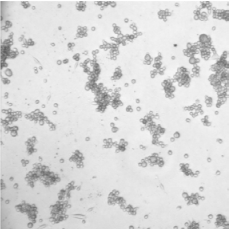
\includegraphics[width=0.3\linewidth]{includes/bhk_original} &
		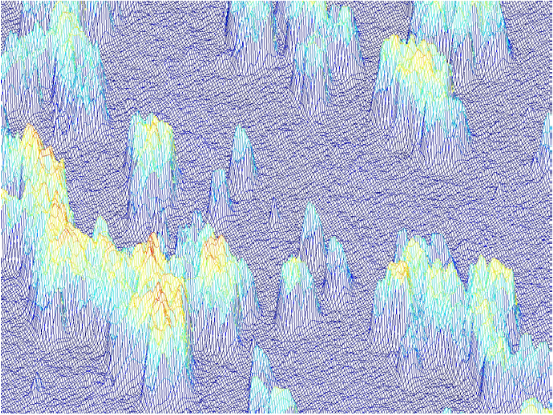
\includegraphics[width=0.3\linewidth]{includes/bhk_lee_rosenfeld} &
		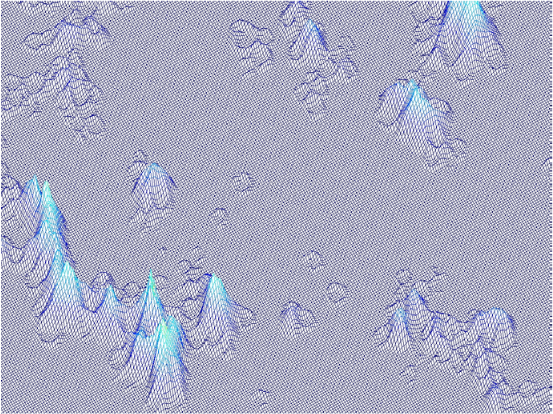
\includegraphics[width=0.3\linewidth]{includes/bhk_binsel_pentland} \\
		Original &
		Lee \& Rosenfeld &
		Bichsel \& Pentland
	\end{tabular}
	\end{center}
	
	\vspace{4em}
	\tiny
	G. Martinez, J.-G. Frerichs, K. Joeris, K. Konstantinov und T.Scheper: Three-Dimensional Shape Estimationof BHK Cell Clusters from a still Image Based on Shape from Shading for In-Situ Microscopy
\end{frame}


\end{document}
